\documentclass[]{article}
\usepackage{lmodern}
\usepackage{amssymb,amsmath}
\usepackage{ifxetex,ifluatex}
\usepackage{fixltx2e} % provides \textsubscript
\ifnum 0\ifxetex 1\fi\ifluatex 1\fi=0 % if pdftex
  \usepackage[T1]{fontenc}
  \usepackage[utf8]{inputenc}
\else % if luatex or xelatex
  \ifxetex
    \usepackage{mathspec}
  \else
    \usepackage{fontspec}
  \fi
  \defaultfontfeatures{Ligatures=TeX,Scale=MatchLowercase}
\fi
% use upquote if available, for straight quotes in verbatim environments
\IfFileExists{upquote.sty}{\usepackage{upquote}}{}
% use microtype if available
\IfFileExists{microtype.sty}{%
\usepackage{microtype}
\UseMicrotypeSet[protrusion]{basicmath} % disable protrusion for tt fonts
}{}
\usepackage[margin=1in]{geometry}
\usepackage{hyperref}
\hypersetup{unicode=true,
            pdftitle={homework 1b},
            pdfauthor={Yi Chen(yc3356)},
            pdfborder={0 0 0},
            breaklinks=true}
\urlstyle{same}  % don't use monospace font for urls
\usepackage{color}
\usepackage{fancyvrb}
\newcommand{\VerbBar}{|}
\newcommand{\VERB}{\Verb[commandchars=\\\{\}]}
\DefineVerbatimEnvironment{Highlighting}{Verbatim}{commandchars=\\\{\}}
% Add ',fontsize=\small' for more characters per line
\usepackage{framed}
\definecolor{shadecolor}{RGB}{248,248,248}
\newenvironment{Shaded}{\begin{snugshade}}{\end{snugshade}}
\newcommand{\KeywordTok}[1]{\textcolor[rgb]{0.13,0.29,0.53}{\textbf{#1}}}
\newcommand{\DataTypeTok}[1]{\textcolor[rgb]{0.13,0.29,0.53}{#1}}
\newcommand{\DecValTok}[1]{\textcolor[rgb]{0.00,0.00,0.81}{#1}}
\newcommand{\BaseNTok}[1]{\textcolor[rgb]{0.00,0.00,0.81}{#1}}
\newcommand{\FloatTok}[1]{\textcolor[rgb]{0.00,0.00,0.81}{#1}}
\newcommand{\ConstantTok}[1]{\textcolor[rgb]{0.00,0.00,0.00}{#1}}
\newcommand{\CharTok}[1]{\textcolor[rgb]{0.31,0.60,0.02}{#1}}
\newcommand{\SpecialCharTok}[1]{\textcolor[rgb]{0.00,0.00,0.00}{#1}}
\newcommand{\StringTok}[1]{\textcolor[rgb]{0.31,0.60,0.02}{#1}}
\newcommand{\VerbatimStringTok}[1]{\textcolor[rgb]{0.31,0.60,0.02}{#1}}
\newcommand{\SpecialStringTok}[1]{\textcolor[rgb]{0.31,0.60,0.02}{#1}}
\newcommand{\ImportTok}[1]{#1}
\newcommand{\CommentTok}[1]{\textcolor[rgb]{0.56,0.35,0.01}{\textit{#1}}}
\newcommand{\DocumentationTok}[1]{\textcolor[rgb]{0.56,0.35,0.01}{\textbf{\textit{#1}}}}
\newcommand{\AnnotationTok}[1]{\textcolor[rgb]{0.56,0.35,0.01}{\textbf{\textit{#1}}}}
\newcommand{\CommentVarTok}[1]{\textcolor[rgb]{0.56,0.35,0.01}{\textbf{\textit{#1}}}}
\newcommand{\OtherTok}[1]{\textcolor[rgb]{0.56,0.35,0.01}{#1}}
\newcommand{\FunctionTok}[1]{\textcolor[rgb]{0.00,0.00,0.00}{#1}}
\newcommand{\VariableTok}[1]{\textcolor[rgb]{0.00,0.00,0.00}{#1}}
\newcommand{\ControlFlowTok}[1]{\textcolor[rgb]{0.13,0.29,0.53}{\textbf{#1}}}
\newcommand{\OperatorTok}[1]{\textcolor[rgb]{0.81,0.36,0.00}{\textbf{#1}}}
\newcommand{\BuiltInTok}[1]{#1}
\newcommand{\ExtensionTok}[1]{#1}
\newcommand{\PreprocessorTok}[1]{\textcolor[rgb]{0.56,0.35,0.01}{\textit{#1}}}
\newcommand{\AttributeTok}[1]{\textcolor[rgb]{0.77,0.63,0.00}{#1}}
\newcommand{\RegionMarkerTok}[1]{#1}
\newcommand{\InformationTok}[1]{\textcolor[rgb]{0.56,0.35,0.01}{\textbf{\textit{#1}}}}
\newcommand{\WarningTok}[1]{\textcolor[rgb]{0.56,0.35,0.01}{\textbf{\textit{#1}}}}
\newcommand{\AlertTok}[1]{\textcolor[rgb]{0.94,0.16,0.16}{#1}}
\newcommand{\ErrorTok}[1]{\textcolor[rgb]{0.64,0.00,0.00}{\textbf{#1}}}
\newcommand{\NormalTok}[1]{#1}
\usepackage{graphicx,grffile}
\makeatletter
\def\maxwidth{\ifdim\Gin@nat@width>\linewidth\linewidth\else\Gin@nat@width\fi}
\def\maxheight{\ifdim\Gin@nat@height>\textheight\textheight\else\Gin@nat@height\fi}
\makeatother
% Scale images if necessary, so that they will not overflow the page
% margins by default, and it is still possible to overwrite the defaults
% using explicit options in \includegraphics[width, height, ...]{}
\setkeys{Gin}{width=\maxwidth,height=\maxheight,keepaspectratio}
\IfFileExists{parskip.sty}{%
\usepackage{parskip}
}{% else
\setlength{\parindent}{0pt}
\setlength{\parskip}{6pt plus 2pt minus 1pt}
}
\setlength{\emergencystretch}{3em}  % prevent overfull lines
\providecommand{\tightlist}{%
  \setlength{\itemsep}{0pt}\setlength{\parskip}{0pt}}
\setcounter{secnumdepth}{0}
% Redefines (sub)paragraphs to behave more like sections
\ifx\paragraph\undefined\else
\let\oldparagraph\paragraph
\renewcommand{\paragraph}[1]{\oldparagraph{#1}\mbox{}}
\fi
\ifx\subparagraph\undefined\else
\let\oldsubparagraph\subparagraph
\renewcommand{\subparagraph}[1]{\oldsubparagraph{#1}\mbox{}}
\fi

%%% Use protect on footnotes to avoid problems with footnotes in titles
\let\rmarkdownfootnote\footnote%
\def\footnote{\protect\rmarkdownfootnote}

%%% Change title format to be more compact
\usepackage{titling}

% Create subtitle command for use in maketitle
\newcommand{\subtitle}[1]{
  \posttitle{
    \begin{center}\large#1\end{center}
    }
}

\setlength{\droptitle}{-2em}

  \title{homework 1b}
    \pretitle{\vspace{\droptitle}\centering\huge}
  \posttitle{\par}
    \author{Yi Chen(yc3356)}
    \preauthor{\centering\large\emph}
  \postauthor{\par}
      \predate{\centering\large\emph}
  \postdate{\par}
    \date{September 6, 2018}


\begin{document}
\maketitle

\subsection{Homework 1}\label{homework-1}

Name: Yi Chen UNI: yc3556 Email:
\href{mailto:yc3556@columbia.edu}{\nolinkurl{yc3556@columbia.edu}}

\subsubsection{1. Exercise 1.9 of BDA}\label{exercise-1.9-of-bda}

\paragraph{(a)}\label{a}

\begin{Shaded}
\begin{Highlighting}[]
\NormalTok{### from 9 am to 4 pm there are total 420 miniutes}

\NormalTok{simulate_process <-}\StringTok{ }\ControlFlowTok{function}\NormalTok{(}\DataTypeTok{times=}\DecValTok{1}\NormalTok{)\{}
        \KeywordTok{set.seed}\NormalTok{(}\DecValTok{1}\NormalTok{)  }\CommentTok{# ensure the result wil not change}
\NormalTok{        number_of_patient <-}\StringTok{ }\KeywordTok{c}\NormalTok{()}
\NormalTok{        number_of_wait <-}\StringTok{ }\KeywordTok{c}\NormalTok{()}
\NormalTok{        average_wait_time <-}\StringTok{ }\KeywordTok{c}\NormalTok{()}
\NormalTok{        office_time <-}\StringTok{ }\KeywordTok{c}\NormalTok{()}
        
        \ControlFlowTok{for}\NormalTok{(a }\ControlFlowTok{in} \DecValTok{1}\OperatorTok{:}\NormalTok{times)\{}
        
        \CommentTok{# simulate the patient: how many patient will come into the office is indepandent to the opration condiation of the office}
\NormalTok{        time <-}\StringTok{ }\DecValTok{0}\NormalTok{ ## time that the office has been operating}
\NormalTok{        patient_time <-}\StringTok{ }\KeywordTok{c}\NormalTok{()}
        \ControlFlowTok{while}\NormalTok{(time }\OperatorTok{<=}\StringTok{ }\DecValTok{420}\NormalTok{)\{}
\NormalTok{                x <-}\StringTok{ }\KeywordTok{rexp}\NormalTok{(}\DataTypeTok{n =} \DecValTok{1}\NormalTok{,}\DataTypeTok{rate =} \DecValTok{1}\OperatorTok{/}\DecValTok{10}\NormalTok{)}
\NormalTok{                time <-}\StringTok{ }\NormalTok{time }\OperatorTok{+}\StringTok{ }\NormalTok{x}
\NormalTok{                patient_time <-}\StringTok{ }\KeywordTok{c}\NormalTok{(patient_time,x)}
\NormalTok{        \}}
\NormalTok{        number_of_patient <-}\StringTok{ }\KeywordTok{c}\NormalTok{(number_of_patient,}\KeywordTok{length}\NormalTok{(patient_time))}
        
        \CommentTok{# simulate the treatment time: a patient that comes before 4 pm would be treated anyway.}
\NormalTok{        treatment_time <-}\StringTok{ }\KeywordTok{c}\NormalTok{()}
        \ControlFlowTok{for}\NormalTok{(i }\ControlFlowTok{in} \DecValTok{1}\OperatorTok{:}\KeywordTok{length}\NormalTok{(patient_time))\{}
\NormalTok{                y <-}\StringTok{ }\KeywordTok{runif}\NormalTok{(}\DataTypeTok{n =} \DecValTok{1}\NormalTok{, }\DataTypeTok{min =} \DecValTok{5}\NormalTok{, }\DataTypeTok{max =} \DecValTok{20}\NormalTok{)}
\NormalTok{                treatment_time <-}\StringTok{ }\KeywordTok{c}\NormalTok{(treatment_time,y)}
\NormalTok{        \}}
        
        
\NormalTok{        doctor_remain_time <-}\StringTok{ }\KeywordTok{c}\NormalTok{(}\DecValTok{0}\NormalTok{,}\DecValTok{0}\NormalTok{,}\DecValTok{0}\NormalTok{)}
\NormalTok{        number_o_wait <-}\StringTok{ }\DecValTok{0}
\NormalTok{        wait_time <-}\StringTok{ }\DecValTok{0}
\NormalTok{        operation_time <-}\StringTok{ }\DecValTok{0}
        \ControlFlowTok{for}\NormalTok{(i }\ControlFlowTok{in} \DecValTok{1}\OperatorTok{:}\KeywordTok{length}\NormalTok{(patient_time))\{}
\NormalTok{                doctor_remain_time <-}\StringTok{ }\NormalTok{doctor_remain_time }\OperatorTok{-}\StringTok{ }\NormalTok{patient_time[i]}
\NormalTok{                operation_time <-}\StringTok{ }\NormalTok{operation_time }\OperatorTok{+}\StringTok{ }\NormalTok{patient_time[i]}
                \ControlFlowTok{if}\NormalTok{(}\KeywordTok{min}\NormalTok{(doctor_remain_time) }\OperatorTok{<=}\StringTok{ }\DecValTok{0}\NormalTok{)\{                        ## do not need to wait}
\NormalTok{                        doctor_remain_time[}\KeywordTok{which}\NormalTok{(doctor_remain_time }\OperatorTok{<}\StringTok{ }\DecValTok{0}\NormalTok{)] <-}\StringTok{ }\DecValTok{0}
\NormalTok{                        doctor_remain_time[}\KeywordTok{which.min}\NormalTok{(doctor_remain_time)] <-}\StringTok{  }\NormalTok{treatment_time[i] }
\NormalTok{                \}}\ControlFlowTok{else}\NormalTok{\{                                                   ## no doctor has finish the job, need to wait}
\NormalTok{                        number_o_wait <-}\StringTok{ }\NormalTok{number_o_wait }\OperatorTok{+}\StringTok{ }\DecValTok{1}
\NormalTok{                        wait_time <-}\StringTok{ }\NormalTok{wait_time }\OperatorTok{+}\StringTok{ }\KeywordTok{min}\NormalTok{(doctor_remain_time)}
\NormalTok{                        operation_time <-}\StringTok{ }\NormalTok{operation_time }\OperatorTok{+}\StringTok{ }\KeywordTok{min}\NormalTok{(doctor_remain_time)}
\NormalTok{                        doctor_remain_time <-}\StringTok{ }\NormalTok{doctor_remain_time }\OperatorTok{-}\StringTok{ }\KeywordTok{min}\NormalTok{(doctor_remain_time)}
\NormalTok{                        doctor_remain_time[}\KeywordTok{which.min}\NormalTok{(doctor_remain_time)] <-}\StringTok{ }\NormalTok{treatment_time[i]}
\NormalTok{                \}}
\NormalTok{        \}}
\NormalTok{        average_wait <-}\StringTok{ }\NormalTok{wait_time }\OperatorTok{/}\StringTok{ }\NormalTok{number_o_wait}
        
\NormalTok{        number_of_wait <-}\StringTok{ }\KeywordTok{c}\NormalTok{(number_of_wait,number_o_wait)}
\NormalTok{        average_wait_time <-}\StringTok{ }\KeywordTok{c}\NormalTok{(average_wait_time,average_wait)}
\NormalTok{        office_time <-}\StringTok{ }\KeywordTok{c}\NormalTok{(office_time,operation_time)}
\NormalTok{\}}
\NormalTok{        result <-}\StringTok{ }\KeywordTok{list}\NormalTok{(number_of_patient,number_of_wait,average_wait_time,office_time)}
        \KeywordTok{return}\NormalTok{(result)}
\NormalTok{\}}
\end{Highlighting}
\end{Shaded}

\begin{Shaded}
\begin{Highlighting}[]
\NormalTok{problem_one <-}\StringTok{ }\KeywordTok{simulate_process}\NormalTok{(}\DecValTok{1}\NormalTok{)}
\KeywordTok{cat}\NormalTok{(}\StringTok{'number of patient:'}\NormalTok{,problem_one[}\DecValTok{1}\NormalTok{][[}\DecValTok{1}\NormalTok{]],}\StringTok{'}\CharTok{\textbackslash{}n}\StringTok{'}\NormalTok{)}
\end{Highlighting}
\end{Shaded}

\begin{verbatim}
## number of patient: 43
\end{verbatim}

\begin{Shaded}
\begin{Highlighting}[]
\KeywordTok{cat}\NormalTok{(}\StringTok{'number of wait:'}\NormalTok{,problem_one[}\DecValTok{2}\NormalTok{][[}\DecValTok{1}\NormalTok{]],}\StringTok{'}\CharTok{\textbackslash{}n}\StringTok{'}\NormalTok{)}
\end{Highlighting}
\end{Shaded}

\begin{verbatim}
## number of wait: 5
\end{verbatim}

\begin{Shaded}
\begin{Highlighting}[]
\KeywordTok{cat}\NormalTok{(}\StringTok{'average waiting time:'}\NormalTok{,problem_one[}\DecValTok{3}\NormalTok{][[}\DecValTok{1}\NormalTok{]],}\StringTok{'}\CharTok{\textbackslash{}n}\StringTok{'}\NormalTok{)}
\end{Highlighting}
\end{Shaded}

\begin{verbatim}
## average waiting time: 3.922496
\end{verbatim}

\begin{Shaded}
\begin{Highlighting}[]
\KeywordTok{cat}\NormalTok{(}\StringTok{'office opetation time:'}\NormalTok{, problem_one[}\DecValTok{4}\NormalTok{][[}\DecValTok{1}\NormalTok{]],}\StringTok{'}\CharTok{\textbackslash{}n}\StringTok{'}\NormalTok{)}
\end{Highlighting}
\end{Shaded}

\begin{verbatim}
## office opetation time: 442.4461
\end{verbatim}

\subparagraph{Note}\label{note}

The total operation time from 9:00 am is 442.45 mins which means the
office really close (stop the last patient's treatment) at approximately
4:23 pm.

\paragraph{(b)}\label{b}

\begin{Shaded}
\begin{Highlighting}[]
\KeywordTok{library}\NormalTok{(}\StringTok{'ggplot2'}\NormalTok{)}
\NormalTok{number_of_patient <-}\StringTok{ }\KeywordTok{simulate_process}\NormalTok{(}\DecValTok{100}\NormalTok{)[}\DecValTok{1}\NormalTok{][[}\DecValTok{1}\NormalTok{]]}
\NormalTok{number_of_wait <-}\StringTok{ }\KeywordTok{simulate_process}\NormalTok{(}\DecValTok{100}\NormalTok{)[}\DecValTok{2}\NormalTok{][[}\DecValTok{1}\NormalTok{]]}
\NormalTok{average_wait_time <-}\StringTok{ }\KeywordTok{simulate_process}\NormalTok{(}\DecValTok{100}\NormalTok{)[}\DecValTok{3}\NormalTok{][[}\DecValTok{1}\NormalTok{]]}
\NormalTok{office_time <-}\StringTok{ }\KeywordTok{simulate_process}\NormalTok{(}\DecValTok{100}\NormalTok{)[}\DecValTok{4}\NormalTok{][[}\DecValTok{1}\NormalTok{]]}
\KeywordTok{qplot}\NormalTok{(number_of_patient)}
\end{Highlighting}
\end{Shaded}

\begin{verbatim}
## `stat_bin()` using `bins = 30`. Pick better value with `binwidth`.
\end{verbatim}

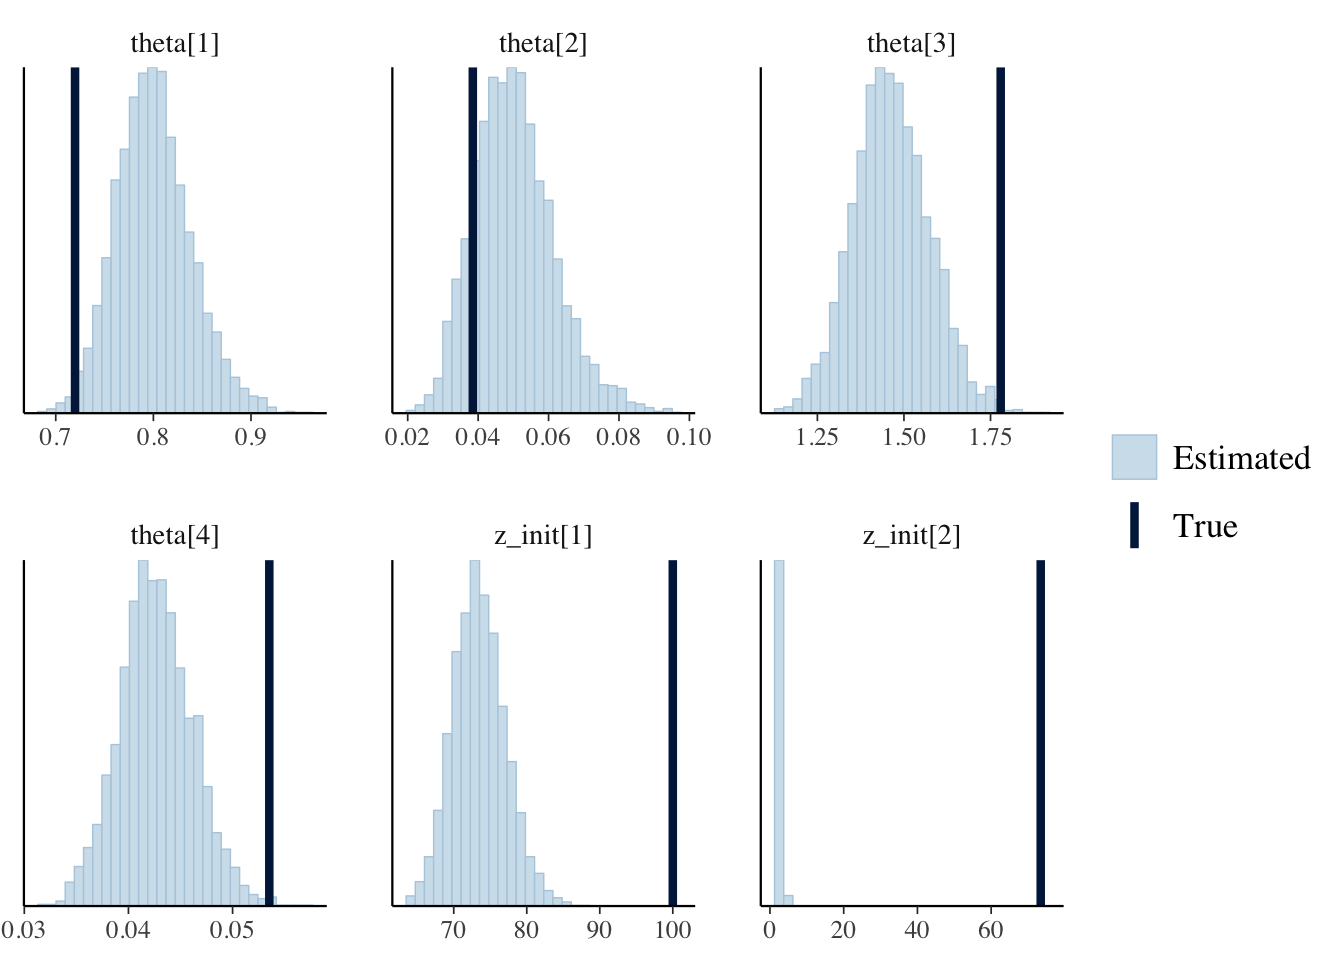
\includegraphics{homework1_files/figure-latex/unnamed-chunk-3-1.pdf}

\begin{Shaded}
\begin{Highlighting}[]
\KeywordTok{qplot}\NormalTok{(number_of_wait)}
\end{Highlighting}
\end{Shaded}

\begin{verbatim}
## `stat_bin()` using `bins = 30`. Pick better value with `binwidth`.
\end{verbatim}

\includegraphics{homework1_files/figure-latex/unnamed-chunk-3-2.pdf}

\begin{Shaded}
\begin{Highlighting}[]
\KeywordTok{qplot}\NormalTok{(average_wait_time)}
\end{Highlighting}
\end{Shaded}

\begin{verbatim}
## `stat_bin()` using `bins = 30`. Pick better value with `binwidth`.
\end{verbatim}

\begin{verbatim}
## Warning: Removed 1 rows containing non-finite values (stat_bin).
\end{verbatim}

\includegraphics{homework1_files/figure-latex/unnamed-chunk-3-3.pdf}

\begin{Shaded}
\begin{Highlighting}[]
\KeywordTok{qplot}\NormalTok{(office_time)}
\end{Highlighting}
\end{Shaded}

\begin{verbatim}
## `stat_bin()` using `bins = 30`. Pick better value with `binwidth`.
\end{verbatim}

\includegraphics{homework1_files/figure-latex/unnamed-chunk-3-4.pdf}

\begin{Shaded}
\begin{Highlighting}[]
\KeywordTok{cat}\NormalTok{(}\StringTok{'median of number of patient:'}\NormalTok{,}\KeywordTok{median}\NormalTok{(number_of_patient),}\StringTok{'}\CharTok{\textbackslash{}n}\StringTok{'}\NormalTok{)}
\end{Highlighting}
\end{Shaded}

\begin{verbatim}
## median of number of patient: 43
\end{verbatim}

\begin{Shaded}
\begin{Highlighting}[]
\KeywordTok{cat}\NormalTok{(}\StringTok{'median of number of wait:'}\NormalTok{,}\KeywordTok{median}\NormalTok{(number_of_wait),}\StringTok{'}\CharTok{\textbackslash{}n}\StringTok{'}\NormalTok{)}
\end{Highlighting}
\end{Shaded}

\begin{verbatim}
## median of number of wait: 4
\end{verbatim}

\begin{Shaded}
\begin{Highlighting}[]
\KeywordTok{cat}\NormalTok{(}\StringTok{'median of average waiting time:'}\NormalTok{,}\KeywordTok{median}\NormalTok{(average_wait_time,}\DataTypeTok{na.rm =}\NormalTok{ T),}\StringTok{'}\CharTok{\textbackslash{}n}\StringTok{'}\NormalTok{)}
\end{Highlighting}
\end{Shaded}

\begin{verbatim}
## median of average waiting time: 3.26708
\end{verbatim}

\begin{Shaded}
\begin{Highlighting}[]
\KeywordTok{cat}\NormalTok{(}\StringTok{'median of office time:'}\NormalTok{, }\KeywordTok{median}\NormalTok{(office_time),}\StringTok{'}\CharTok{\textbackslash{}n}\StringTok{'}\NormalTok{)}
\end{Highlighting}
\end{Shaded}

\begin{verbatim}
## median of office time: 441.0266
\end{verbatim}

\begin{Shaded}
\begin{Highlighting}[]
\KeywordTok{cat}\NormalTok{(}\StringTok{'the 50% interval of the number of patient is:['}\NormalTok{,}\KeywordTok{quantile}\NormalTok{(number_of_patient,}\DataTypeTok{probs =} \FloatTok{0.25}\NormalTok{),}\StringTok{','}\NormalTok{,}\KeywordTok{quantile}\NormalTok{(number_of_patient,}\DataTypeTok{probs =} \FloatTok{0.75}\NormalTok{),}\StringTok{']}\CharTok{\textbackslash{}n}\StringTok{'}\NormalTok{)}
\end{Highlighting}
\end{Shaded}

\begin{verbatim}
## the 50% interval of the number of patient is:[ 38 , 48 ]
\end{verbatim}

\begin{Shaded}
\begin{Highlighting}[]
\KeywordTok{cat}\NormalTok{(}\StringTok{'the 50% interval of the number of wait is:'}\NormalTok{,}\StringTok{'['}\NormalTok{,}\KeywordTok{quantile}\NormalTok{(number_of_wait,}\DataTypeTok{probs =} \FloatTok{0.25}\NormalTok{),}\StringTok{','}\NormalTok{,}\KeywordTok{quantile}\NormalTok{(number_of_wait,}\DataTypeTok{probs =} \FloatTok{0.75}\NormalTok{),}\StringTok{']}\CharTok{\textbackslash{}n}\StringTok{'}\NormalTok{)}
\end{Highlighting}
\end{Shaded}

\begin{verbatim}
## the 50% interval of the number of wait is: [ 2 , 6 ]
\end{verbatim}

\begin{Shaded}
\begin{Highlighting}[]
\KeywordTok{cat}\NormalTok{(}\StringTok{'the 50% interval of the average wait time is:'}\NormalTok{,}\StringTok{'['}\NormalTok{,}\KeywordTok{quantile}\NormalTok{(average_wait_time,}\DataTypeTok{probs =} \FloatTok{0.25}\NormalTok{,}\DataTypeTok{na.rm =}\NormalTok{ T),}\StringTok{','}\NormalTok{,}\KeywordTok{quantile}\NormalTok{(average_wait_time,}\DataTypeTok{probs =} \FloatTok{0.75}\NormalTok{,}\DataTypeTok{na.rm =}\NormalTok{ T),}\StringTok{']}\CharTok{\textbackslash{}n}\StringTok{'}\NormalTok{)}
\end{Highlighting}
\end{Shaded}

\begin{verbatim}
## the 50% interval of the average wait time is: [ 2.420231 , 4.258315 ]
\end{verbatim}

\begin{Shaded}
\begin{Highlighting}[]
\KeywordTok{cat}\NormalTok{(}\StringTok{'the 50% interval of the number of office time is:'}\NormalTok{,}\StringTok{'['}\NormalTok{,}\KeywordTok{quantile}\NormalTok{(office_time,}\DataTypeTok{probs =} \FloatTok{0.25}\NormalTok{),}\StringTok{','}\NormalTok{,}\KeywordTok{quantile}\NormalTok{(office_time,}\DataTypeTok{probs =} \FloatTok{0.75}\NormalTok{),}\StringTok{']}\CharTok{\textbackslash{}n}\StringTok{'}\NormalTok{)}
\end{Highlighting}
\end{Shaded}

\begin{verbatim}
## the 50% interval of the number of office time is: [ 431.8638 , 452.378 ]
\end{verbatim}

\paragraph{Note}\label{note-1}

The medain of total office based on 100 simulation is 441.03 which means
the median office close time is 4:21 pm. And the 50\% interval of the
office time is {[}431.86,452.38{]} which means the 50\% intercal of
close time is 4:12 pm to 4:32 pm.

\subsubsection{1. Fitting a simple model to simulate
data}\label{fitting-a-simple-model-to-simulate-data}

\paragraph{(a) stan model}\label{a-stan-model}

\begin{Shaded}
\begin{Highlighting}[]
\KeywordTok{library}\NormalTok{(}\StringTok{"rstan"}\NormalTok{)}
\KeywordTok{options}\NormalTok{(}\DataTypeTok{mc.cores =}\NormalTok{ parallel}\OperatorTok{::}\KeywordTok{detectCores}\NormalTok{())}
\KeywordTok{rstan_options}\NormalTok{(}\DataTypeTok{auto_write =} \OtherTok{TRUE}\NormalTok{)}
\end{Highlighting}
\end{Shaded}

\paragraph{(b) fake data}\label{b-fake-data}

\begin{Shaded}
\begin{Highlighting}[]
\KeywordTok{set.seed}\NormalTok{(}\DecValTok{10}\NormalTok{)}
\NormalTok{N =}\StringTok{ }\DecValTok{100}
\NormalTok{a <-}\StringTok{ }\DecValTok{4}
\NormalTok{b <-}\StringTok{ }\DecValTok{3}
\NormalTok{sigma <-}\StringTok{ }\DecValTok{2}
\NormalTok{x <-}\StringTok{ }\KeywordTok{runif}\NormalTok{(}\DataTypeTok{n =}\NormalTok{ N,}\DataTypeTok{min =} \DecValTok{0}\NormalTok{,}\DataTypeTok{max =} \DecValTok{10}\NormalTok{)}
\NormalTok{y <-}\StringTok{ }\NormalTok{a}\OperatorTok{*}\StringTok{ }\KeywordTok{sin}\NormalTok{(b}\OperatorTok{*}\NormalTok{x)}\OperatorTok{+}\StringTok{ }\KeywordTok{rnorm}\NormalTok{(N,}\DecValTok{0}\NormalTok{,sigma)}
\KeywordTok{hist}\NormalTok{(x,}\DataTypeTok{breaks =} \DecValTok{30}\NormalTok{)}
\end{Highlighting}
\end{Shaded}

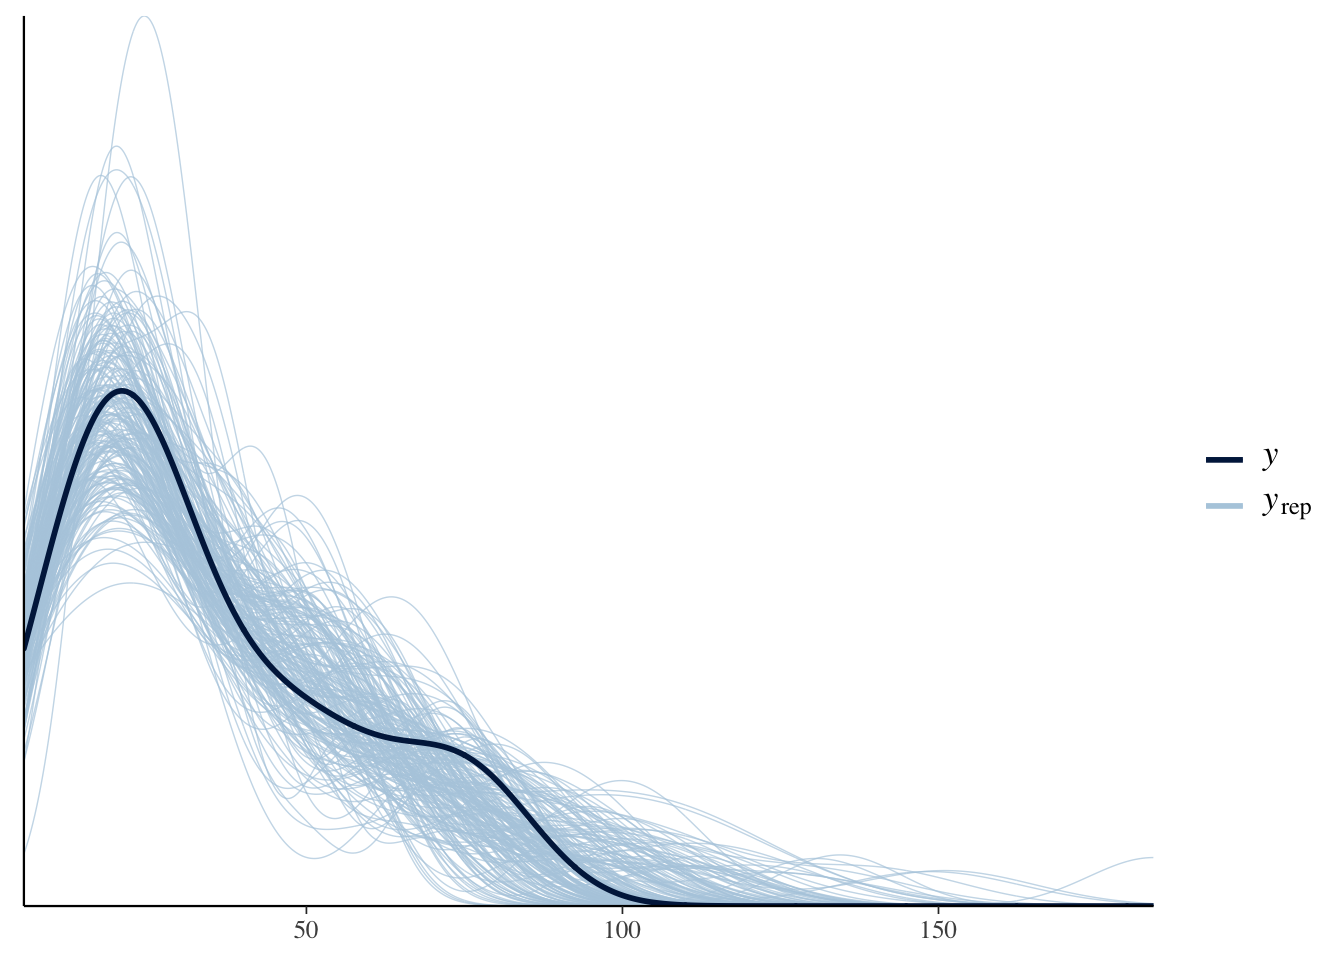
\includegraphics{homework1_files/figure-latex/unnamed-chunk-5-1.pdf}

\begin{Shaded}
\begin{Highlighting}[]
\KeywordTok{hist}\NormalTok{(y,}\DataTypeTok{breaks =} \DecValTok{30}\NormalTok{)}
\end{Highlighting}
\end{Shaded}

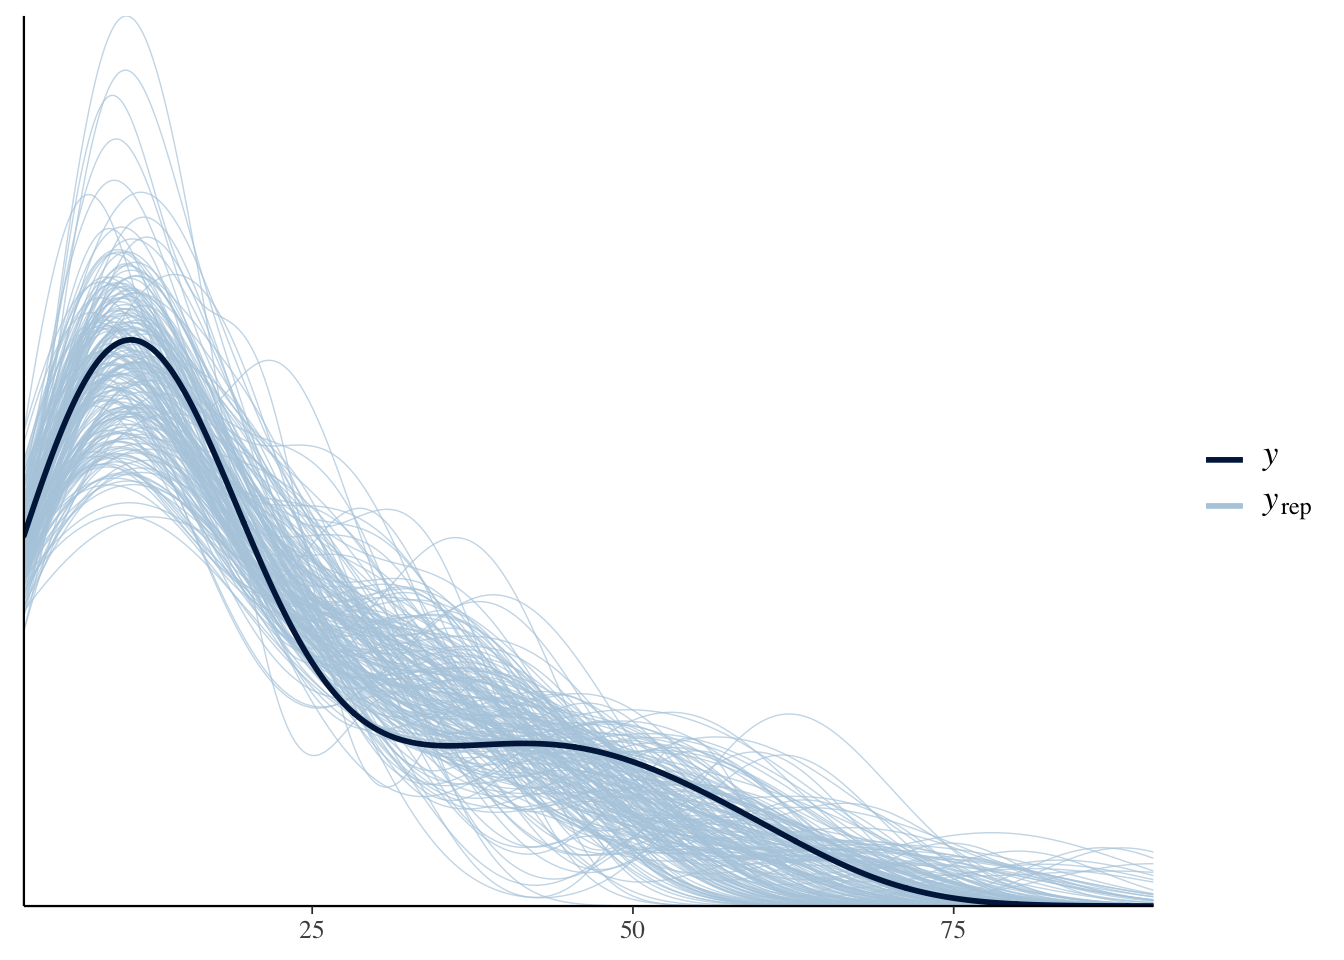
\includegraphics{homework1_files/figure-latex/unnamed-chunk-5-2.pdf}

\paragraph{(c) fit the model}\label{c-fit-the-model}

Following is the copy of the stan file which called: `homework1b.stan'

data \{

int N;

vector{[}N{]} y;

vector{[}N{]} x;

\}

parameters \{

real a;

real b;

real \(\sigma\);

\}

model \{

y \textasciitilde{} normal(a \emph{sin(b}x), \(\sigma\));

\}

\begin{Shaded}
\begin{Highlighting}[]
\NormalTok{data =}\StringTok{ }\KeywordTok{list}\NormalTok{(}\DataTypeTok{y=}\NormalTok{y,}\DataTypeTok{x=}\NormalTok{x,}\DataTypeTok{N=}\NormalTok{N)}
\NormalTok{fit <-}\StringTok{ }\KeywordTok{stan}\NormalTok{(}\StringTok{'homework1b.stan'}\NormalTok{,}\DataTypeTok{data =}\NormalTok{ data,}\DataTypeTok{seed =} \DecValTok{1}\NormalTok{,)}
\KeywordTok{print}\NormalTok{(fit)}
\end{Highlighting}
\end{Shaded}

\begin{verbatim}
## Inference for Stan model: homework1b.
## 4 chains, each with iter=2000; warmup=1000; thin=1; 
## post-warmup draws per chain=1000, total post-warmup draws=4000.
## 
##          mean se_mean   sd    2.5%     25%     50%     75%   97.5% n_eff
## a        1.98    2.44 3.46   -4.33    1.42    3.86    4.09    4.51     2
## b        1.49    1.83 2.59   -3.00    1.47    2.98    2.99    3.01     2
## sigma    1.97    0.00 0.14    1.71    1.87    1.96    2.06    2.28  3264
## lp__  -116.25    0.03 1.23 -119.36 -116.82 -115.94 -115.34 -114.85  2176
##         Rhat
## a      13.10
## b     220.97
## sigma   1.00
## lp__    1.00
## 
## Samples were drawn using NUTS(diag_e) at Fri Sep 14 08:27:16 2018.
## For each parameter, n_eff is a crude measure of effective sample size,
## and Rhat is the potential scale reduction factor on split chains (at 
## convergence, Rhat=1).
\end{verbatim}

we can see that the true value a = 4 , b = 3, sigma = 2 are
approximately recorved. Especially, the median of the estimation is very
close to the true value. But, the R hat is not fit very well.

\paragraph{(d) simulated data and fitted
model}\label{d-simulated-data-and-fitted-model}

\begin{Shaded}
\begin{Highlighting}[]
\NormalTok{## if we fit the model with mean}
\NormalTok{results <-}\StringTok{ }\KeywordTok{extract}\NormalTok{(fit)}
\NormalTok{number_of_simulation <-}\StringTok{ }\KeywordTok{length}\NormalTok{(results}\OperatorTok{$}\NormalTok{a)}
\KeywordTok{plot}\NormalTok{(x,y)}
\NormalTok{a_mean <-}\StringTok{ }\KeywordTok{mean}\NormalTok{(results}\OperatorTok{$}\NormalTok{a)}
\NormalTok{b_mean <-}\StringTok{ }\KeywordTok{mean}\NormalTok{(results}\OperatorTok{$}\NormalTok{b)}
\NormalTok{a_median <-}\StringTok{ }\KeywordTok{median}\NormalTok{(results}\OperatorTok{$}\NormalTok{a)}
\NormalTok{b_median <-}\StringTok{ }\KeywordTok{median}\NormalTok{(results}\OperatorTok{$}\NormalTok{b)}
\KeywordTok{curve}\NormalTok{(a_mean}\OperatorTok{*}\KeywordTok{sin}\NormalTok{(b_mean}\OperatorTok{*}\NormalTok{x),}\DataTypeTok{add =}\NormalTok{ T,}\DataTypeTok{col=}\StringTok{'red'}\NormalTok{)}
\KeywordTok{curve}\NormalTok{(a_median}\OperatorTok{*}\KeywordTok{sin}\NormalTok{(b_median}\OperatorTok{*}\NormalTok{x),}\DataTypeTok{add =}\NormalTok{ T,}\DataTypeTok{col=}\StringTok{'blue'}\NormalTok{)}
\end{Highlighting}
\end{Shaded}

\includegraphics{homework1_files/figure-latex/unnamed-chunk-7-1.pdf}

Note: The red the line fitted model based on the mean and the blue line
is the fitted model based on the median. Cleary, the medain is a better
estimation.

\begin{Shaded}
\begin{Highlighting}[]
\CommentTok{# explore more}
\KeywordTok{plot}\NormalTok{(x,y)}
\ControlFlowTok{for}\NormalTok{(i }\ControlFlowTok{in} \KeywordTok{sample}\NormalTok{(number_of_simulation,}\DecValTok{10}\NormalTok{))\{}
\NormalTok{        a_post <-}\StringTok{ }\NormalTok{results}\OperatorTok{$}\NormalTok{a[i]}
\NormalTok{        b_post <-}\StringTok{ }\NormalTok{results}\OperatorTok{$}\NormalTok{b[i]}
        \KeywordTok{curve}\NormalTok{(a_post}\OperatorTok{*}\KeywordTok{sin}\NormalTok{(b_post}\OperatorTok{*}\NormalTok{x),}\DataTypeTok{add =} \OtherTok{TRUE}\NormalTok{,}\DataTypeTok{col=}\StringTok{'blue'}\NormalTok{,}\DataTypeTok{lwd=}\FloatTok{0.5}\NormalTok{)}
\NormalTok{\}}
\end{Highlighting}
\end{Shaded}

\includegraphics{homework1_files/figure-latex/unnamed-chunk-8-1.pdf}

As we can see that: the result shows that the model fit the data very
well.

\paragraph{(e) report}\label{e-report}

There are some points that I feel confused: 1. the result of the
estimation is not robust. The esitimations change a lot. 2. Why median
is a better estimation all the time?

\subsubsection{3. jitt1b}\label{jitt1b}

\paragraph{problem 2}\label{problem-2}

\begin{Shaded}
\begin{Highlighting}[]
\NormalTok{jitt_1b_}\DecValTok{2}\NormalTok{ <-}\StringTok{ }\ControlFlowTok{function}\NormalTok{(}\DataTypeTok{times=}\DecValTok{1}\NormalTok{)\{}
        \KeywordTok{set.seed}\NormalTok{(}\DecValTok{1}\NormalTok{)}
\NormalTok{        result <-}\StringTok{ }\KeywordTok{c}\NormalTok{()}
        \ControlFlowTok{for}\NormalTok{(i }\ControlFlowTok{in} \DecValTok{1}\OperatorTok{:}\NormalTok{times)\{}
\NormalTok{          x <-}\StringTok{ }\KeywordTok{rnorm}\NormalTok{(}\DataTypeTok{n=}\DecValTok{1}\NormalTok{,}\DataTypeTok{mean =} \DecValTok{0}\NormalTok{,}\DataTypeTok{sd=}\DecValTok{1}\NormalTok{)}
\NormalTok{          y <-}\StringTok{ }\KeywordTok{rnorm}\NormalTok{(}\DataTypeTok{n=}\DecValTok{1}\NormalTok{,}\DataTypeTok{mean =} \DecValTok{0}\NormalTok{,}\DataTypeTok{sd=}\DecValTok{1}\NormalTok{)}
          \ControlFlowTok{if}\NormalTok{(}\KeywordTok{abs}\NormalTok{(x)}\OperatorTok{>}\DecValTok{2}\OperatorTok{*}\KeywordTok{abs}\NormalTok{(y))\{}
\NormalTok{                  result <-}\StringTok{ }\KeywordTok{c}\NormalTok{(result,}\OtherTok{TRUE}\NormalTok{)}
\NormalTok{          \}}\ControlFlowTok{else}\NormalTok{\{}
\NormalTok{                  result <-}\StringTok{ }\KeywordTok{c}\NormalTok{(result,}\OtherTok{FALSE}\NormalTok{)}
\NormalTok{          \}}
\NormalTok{        \}}
        \KeywordTok{return}\NormalTok{(}\KeywordTok{mean}\NormalTok{(result))}
\NormalTok{\}}
\KeywordTok{print}\NormalTok{(}\KeywordTok{jitt_1b_2}\NormalTok{(}\DecValTok{100000}\NormalTok{))}
\end{Highlighting}
\end{Shaded}

\begin{verbatim}
## [1] 0.2936
\end{verbatim}

\paragraph{problem 3}\label{problem-3}

\begin{Shaded}
\begin{Highlighting}[]
\KeywordTok{print}\NormalTok{(}\DecValTok{1}\OperatorTok{-}\StringTok{ }\KeywordTok{pnorm}\NormalTok{(}\OperatorTok{-}\DecValTok{7}\OperatorTok{/}\DecValTok{14}\NormalTok{))}
\end{Highlighting}
\end{Shaded}

\begin{verbatim}
## [1] 0.6914625
\end{verbatim}


\end{document}
